% 2001 年春季上海卷第 20 题：长方体中的点与平面
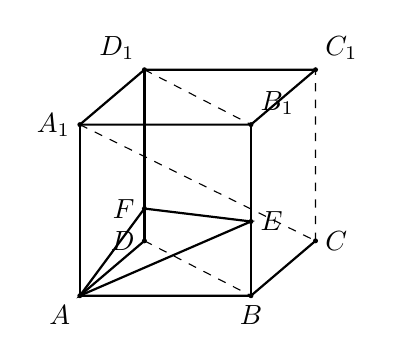
\begin{tikzpicture}[>=stealth, scale=0.82]
  \coordinate (A) at (0,0);
  \coordinate (B) at (2.65,0);
  \coordinate (C) at (3.65,0.85);
  \coordinate (D) at (1,0.85);
  \coordinate (A1) at (0,2.65);
  \coordinate (B1) at (2.65,2.65);
  \coordinate (C1) at (3.65,3.5);
  \coordinate (D1) at (1,3.5);
  \coordinate (E) at (2.65,1.15);
  \coordinate (F) at (1,1.35);

  \draw[thick] (A)--(B)--(C);
  \draw[thick] (A)--(D);
  \draw[thick] (A1)--(B1)--(C1);
  \draw[thick] (A1)--(D1)--(C1);
  \draw[thick] (A)--(A1) (B)--(B1) (D)--(D1);
  \draw[dashed] (C)--(C1) (D1)--(B1) (D)--(B);
  \draw[thick] (A)--(E)--(F)--cycle;
  \draw[dashed] (A1)--(C);

  \fill (A) circle (1.1pt) node[below left] {$A$};
  \fill (B) circle (1.1pt) node[below] {$B$};
  \fill (C) circle (1.1pt) node[right] {$C$};
  \fill (D) circle (1.1pt) node[left] {$D$};
  \fill (A1) circle (1.1pt) node[left] {$A_1$};
  \fill (B1) circle (1.1pt) node[above right] {$B_1$};
  \fill (C1) circle (1.1pt) node[above right] {$C_1$};
  \fill (D1) circle (1.1pt) node[above left] {$D_1$};
  \fill (E) circle (1.1pt) node[right] {$E$};
  \fill (F) circle (1.1pt) node[left] {$F$};
\end{tikzpicture}
